\beamersection{Graphen}

\subsection{Knoten}

\begin{Frame}{Wofür Knoten?}
  \begin{itemize}
    \item \alert{Wir können jetzt alles zeichnen.}
    \item Viele Zeichnungen basieren auf Graphen,
      bestehen also aus Knoten und Kanten.
      \begin{itemize}
        \item Automaten
        \item UML-Diagramme
        \item Stoffwechselwege
        \item Ablaufdiagramme
      \end{itemize}
    \item Solche Diagramme mit Kreisen und Linien zu zeichnen erzeugt
      \alert{unübersichtlichen und schlecht wartbaren} \LaTeX-Code.
  \end{itemize}
\end{Frame}

\begin{Frame}{Ein zweites Beispiel}
  \tikzexample{
    [io/.style={trapezium, trapezium left angle=70, trapezium right angle=110, fill=magenta!10, draw=magenta},
    op/.style={rectangle, fill=orange!10, draw=orange},
    cn/.style={diamond, aspect=2, inner sep=2pt, fill=red!10, draw=red},
    node distance=5mm, thick]
    \node[io] (in) {Eingabe $a,b$};
    \node[op, below=of in] (div) {$r=a \mod b$};
    \node[op, below=of div] (set) {$a=b,\ b=r$};
    \node[cn, below=of set] (cond) {$b=0?$};
    \node[io, below=of cond] (out) {Ausgabe $a$};
    %
    \path[->]
      (in) edge (div)
      (div) edge (set)
      (set) edge (cond)
      (cond) edge node[right] {Ja} (out);
    \draw[->] (cond) -- node[below] {Nein} ++(1.5,0) |- (div);
  }
\end{Frame}

\begin{Frame}[fragile]{Knoten sind Pfadelemente.}
  \begin{columns}
    \column{30mm}
      \tikzexample[left]{
        \path
          (0,4) node {Eingabe $a,b$}
          (0,3) node {$r=a \mod b$}
          (0,2) node {$a=b,\ b=r$}
          (0,1) node {$b=0?$}
          (0,0) node {Ausgabe $a$};
      }
    \column{58mm}
      \begin{lstlisting}[gobble=8]
        \path
          (0,4) node {Eingabe $a,b$}
          (0,3) node {$r=a \mod b$}
          (0,2) node {$a=b,\ b=r$}
          (0,1) node {$b=0?$}
          (0,0) node {Ausgabe $a$};
      \end{lstlisting}
  \end{columns}
\end{Frame}

\begin{Frame}[fragile]{Knoten haben einen eigenen Befehl.}
  \begin{columns}
    \column{30mm}
      \tikzexample[left]{
        \node at (0,4) {Eingabe $a,b$};
        \node at (0,3) {$r=a \mod b$};
        \node at (0,2) {$a=b,\ b=r$};
        \node at (0,1) {$b=0?$};
        \node at (0,0) {Ausgabe $a$};
      }
    \column{58mm}
      \begin{lstlisting}[gobble=8]
        \node at (0,4) {...};
        \node at (0,3) {...};
        \node at (0,2) {...};
        \node at (0,1) {...};
        \node at (0,0) {...};
      \end{lstlisting}
  \end{columns}
\end{Frame}

\begin{Frame}[fragile]{Knoten haben Stile.}{Ein- und Ausgabe}
  \tikzexample{[io/.style={trapezium,
      trapezium left angle=70,
      trapezium right angle=110,
      fill=magenta!10, draw=magenta}, thick]
    \node[io] {Eingabe $a,b$};
  }

  \xxx

  \begin{lstlisting}[gobble=4]
    \begin{tikzpicture}[io/.style={trapezium,
        trapezium left angle=70,
        trapezium right angle=110,
        fill=magenta!10, draw=magenta}, thick]
      \node[io] {Eingabe $a,b$};
    \end{tikzpicture}
  \end{lstlisting}
\end{Frame}

\begin{Frame}[fragile]{Knoten haben Stile.}{Operationen}
  \tikzexample{[op/.style={rectangle, fill=orange!10, draw=orange}, thick]
    \node[op] {$r=a \mod b$};
  }

  \xxx

  \begin{lstlisting}[gobble=4]
    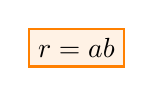
\begin{tikzpicture}[op/.style={rectangle,
        fill=orange!10, draw=orange}, thick]
      \node[op] {$r=a \mod b$};
    \end{tikzpicture}
  \end{lstlisting}
\end{Frame}

\begin{Frame}[fragile]{Knoten haben Stile.}{Entscheidungen}
  \tikzexample{[cn/.style={diamond, aspect=2, inner sep=2pt, fill=red!10, draw=red}, thick]
    \node[cn] {$b=0?$};
  }

  \xxx

  \begin{lstlisting}[gobble=4]
    \begin{tikzpicture}[cn/.style={diamond,
        aspect=2, inner sep=2pt,
        fill=red!10, draw=red}, thick]
      \node[cn] {$b=0?$};
    \end{tikzpicture}
  \end{lstlisting}
\end{Frame}

\begin{Frame}[t,fragile]{Knoten haben Namen.}
  \xxx\xxx
  \begin{columns}[T]
    \column{30mm}
      \tikzexample[left]{[io/.style={trapezium, trapezium left angle=70, trapezium right angle=110, fill=magenta!10, draw=magenta},
        op/.style={rectangle, fill=orange!10, draw=orange},
        cn/.style={diamond, aspect=2, inner sep=2pt, fill=red!10, draw=red}, thick]
        \node[io] at (0,4) (in) {Eingabe $a,b$};
        \node[op] at (0,3) (div) {$r=a \mod b$};
        \node[op] at (0,2) (set) {$a=b,\ b=r$};
        \node[cn] at (0,1) (cond) {$b=0?$};
        \node[io] at (0,0) (out) {Ausgabe $a$};
      }
    \column{55mm}
      \xxx
      \begin{lstlisting}[gobble=8]
        \node[io] at (0,4)
          (in) {Eingabe $a,b$};
        \node[op] at (0,3)
          (div) {$r=a \mod b$};
        \node[op] at (0,2)
          (set) {$a=b,\ b=r$};
        \node[cn] at (0,1)
          (cond) {$b=0?$};
        \node[io] at (0,0)
          (out) {Ausgabe $a$};
      \end{lstlisting}
  \end{columns}
\end{Frame}

\begin{Frame}[t,fragile]{Knoten relativ positionieren}
  \xxx\xxx
  \begin{columns}[T]
    \column{30mm}
      \tikzexample[left]{[io/.style={trapezium, trapezium left angle=70, trapezium right angle=110, fill=magenta!10, draw=magenta},
        op/.style={rectangle, fill=orange!10, draw=orange},
        cn/.style={diamond, aspect=2, inner sep=2pt, fill=red!10, draw=red}, thick, node distance=5mm]
        \node[io] (in) {Eingabe $a,b$};
        \node[op, below=of in] (div) {$r=a \mod b$};
        \node[op, below=of div] (set) {$a=b,\ b=r$};
        \node[cn, below=of set] (cond) {$b=0?$};
        \node[io, below=of cond] (out) {Ausgabe $a$};
      }
    \column{55mm}
      \xxx
      \begin{lstlisting}[gobble=8]
        \node[io]
          (in) {Eingabe $a,b$};
        \node[op, below=of in]
          (div) {$r=a \mod b$};
        \node[op, below=of div]
          (set) {$a=b,\ b=r$};
        \node[cn, below=of set]
          (cond) {$b=0?$};
        \node[io, below=of cond]
          (out) {Ausgabe $a$};
      \end{lstlisting}
  \end{columns}
\end{Frame}

\begin{Frame}[t,fragile]{Kanten}
  \xxx\xxx
  \begin{columns}[T]
    \column{30mm}
      \tikzexample[left]{[io/.style={trapezium, trapezium left angle=70, trapezium right angle=110, fill=magenta!10, draw=magenta},
        op/.style={rectangle, fill=orange!10, draw=orange},
        cn/.style={diamond, aspect=2, inner sep=2pt, fill=red!10, draw=red}, thick, node distance=5mm]
        \node[io] (in) {Eingabe $a,b$};
        \node[op, below=of in] (div) {$r=a \mod b$};
        \node[op, below=of div] (set) {$a=b,\ b=r$};
        \node[cn, below=of set] (cond) {$b=0?$};
        \node[io, below=of cond] (out) {Ausgabe $a$};
        %
        \path[->]
          (in) edge (div)
          (div) edge (set)
          (set) edge (cond)
          (cond) edge (out);
      }
    \column{55mm}
      \xxx
      \begin{lstlisting}[gobble=8]
        \path[->]
          (in) edge (div)
          (div) edge (set)
          (set) edge (cond)
          (cond) edge (out);
      \end{lstlisting}
  \end{columns}
\end{Frame}

\begin{Frame}[t,fragile]{Ein Pfad um die Ecke}
  \xxx\xxx
  \begin{columns}[T]
    \column{35mm}
      \tikzexample[left]{[io/.style={trapezium, trapezium left angle=70, trapezium right angle=110, fill=magenta!10, draw=magenta},
        op/.style={rectangle, fill=orange!10, draw=orange},
        cn/.style={diamond, aspect=2, inner sep=2pt, fill=red!10, draw=red}, thick, node distance=5mm]
        \node[io] (in) {Eingabe $a,b$};
        \node[op, below=of in] (div) {$r=a \mod b$};
        \node[op, below=of div] (set) {$a=b,\ b=r$};
        \node[cn, below=of set] (cond) {$b=0?$};
        \node[io, below=of cond] (out) {Ausgabe $a$};
        %
        \path[->]
          (in) edge (div)
          (div) edge (set)
          (set) edge (cond)
          (cond) edge (out);
        \draw[->] (cond) -- ++(1.5,0) |- (div);
      }
    \column{50mm}
      \xxx
      \begin{lstlisting}[gobble=8]
        \draw[->]
          (cond) -- ++(1.5,0)
                 |- (div);
      \end{lstlisting}
  \end{columns}
\end{Frame}

\begin{Frame}[t,fragile]{Beschriftete Kanten}{\texttt{examples/knoten.tex}}
  \xxx\xxx
  \begin{columns}[T]
    \column{35mm}
      \tikzexample[left]{[io/.style={trapezium, trapezium left angle=70, trapezium right angle=110, fill=magenta!10, draw=magenta},
        op/.style={rectangle, fill=orange!10, draw=orange},
        cn/.style={diamond, aspect=2, inner sep=2pt, fill=red!10, draw=red}, thick, node distance=5mm]
        \node[io] (in) {Eingabe $a,b$};
        \node[op, below=of in] (div) {$r=a \mod b$};
        \node[op, below=of div] (set) {$a=b,\ b=r$};
        \node[cn, below=of set] (cond) {$b=0?$};
        \node[io, below=of cond] (out) {Ausgabe $a$};
        %
        \path[->]
          (in) edge (div)
          (div) edge (set)
          (set) edge (cond)
          (cond) edge node[right] {Ja} (out);
        \draw[->] (cond) -- node[below] {Nein} ++(1.5,0) |- (div);
      }
    \column{50mm}
      \xxx
      \begin{lstlisting}[gobble=8]
        \path[->]
          (cond) edge
            node[right] {Ja}
              (out);
        \draw[->] (cond) --
          node[below] {Nein}
            ++(1.5,0) |- (div);
      \end{lstlisting}
  \end{columns}
\end{Frame}

\subsection{Automaten}

\begin{Frame}[fragile]{Automaten}
  \tikzexample{[auto, thick]
    \node[initial,state] (q0) {$q_0$};
    \visible<2->{\node[state, right=of q0] (q1) {$q_1$};}
    \visible<3->{\node[state, accepting, right=of q1] (q2) {$q_2$};}
    \visible<2->{\path
      (q0) edge[->] node {0} (q1)
      (q1) edge[->, loop above] node {0} ();}
    \visible<3->{\path
      (q1) edge[->, bend left] node {1} (q2)
      (q2) edge[->, bend left] node {0} (q1);}
  }

  \xxx

  \begin{lstlisting}[gobble=4,escapechar=\%]
    \tikz[auto, thick]{
      %\pause[1]%\node[initial, state] (q0) {$q_0$};            %\onslide%
      %\pause[2]%\node[state, right=of q0] (q1) {$q_1$};        %\onslide%
      %\pause[3]%\node[state, accepting, right=of q1]           %\onslide%
      %\pause[3]%  (q2) {$q_2$};                                %\onslide%
      %\pause[2]%\path (q0) edge[->] node {0} (q1)              %\onslide%
      %\pause[2]%      (q1) edge[->, loop above] node {0} ()    %\onslide%
      %\pause[3]%           edge[->, bend left] node {1} (q2)   %\onslide%
      %\pause[3]%      (q2) edge[->, bend left] node {0} (q1)%\pause[2]%;%\onslide%}
  \end{lstlisting}
\end{Frame}

\subsection{Bäume}

\begin{Frame}[fragile]{Bäume}{\texttt{examples/baum.tex}}
  \begin{columns}
    \column{42mm}
      \tikzexample[left]{[
        every node/.style={draw,circle,inner sep=0pt,minimum width=15pt},%
        edge from parent/.style={},%
        level/.style={sibling distance=20mm/#1},%
        level distance=10mm, thick]
        \node[coordinate] (root) {}
          child { child child }
          child { child child };
        %
        \node at (root) (a) {a};
        \visible<2->{\node at (root-1) (b) {b};}
        \visible<4->{\node at (root-2) (e) {e};}
        \visible<3->{\node at (root-1-1) (c) {c};}
        \visible<3->{\node at (root-1-2) (d) {d};}
        \visible<5->{\node at (root-2-1) (f) {f};}
        \visible<5->{\node at (root-2-2) (g) {g};}
        \visible<2->{\path (a) edge (b);}
        \visible<4->{\path (a) edge (e);}
        \visible<3->{\path (b) edge (c)
                       edge (d);}
        \visible<5->{\path (e) edge (f)
                       edge (g);}
      }

    \column{52mm}

    \begin{lstlisting}[gobble=6,escapechar=\%]
      %\pause[1]%\node {a}                %\onslide%
      %\pause[2]%  child { node {b}       %\onslide%
      %\pause[3]%    child { node {c} }   %\onslide%
      %\pause[3]%    child { node {d} }   %\onslide%
      %\pause[2]%  }                      %\onslide%
      %\pause[4]%  child { node {e}       %\onslide%
      %\pause[5]%    child { node {f} }   %\onslide%
      %\pause[5]%    child { node {g} }   %\onslide%
      %\pause[4]%  }%\onslide%;
    \end{lstlisting}
  \end{columns}
\end{Frame}

